\documentclass[t]{beamer}

\mode<presentation>
{
    \usetheme{rwthsimple}
    \setbeamercovered{transparent = 0}
}

\setbeamertemplate{section in toc shaded}[default][30]
\setbeamertemplate{subsection in toc shaded}[default][30]

\usepackage{enumerate}
\usepackage{xcolor}
\usepackage{url}
\usepackage{hyperref}
\usepackage{subfigure}
\usepackage{ulem}
\usepackage{amssymb}
\usepackage{amsmath}
\usepackage{pgfplots}
\usepackage{tikz}
\usetikzlibrary{arrows.new}
\usetikzlibrary{fadings}

% \pgfplotsset{compat=1.9}

\title{Neural Codes for Image Retrieval}
\author{David Stutz}
\date{July 22, 2015}

\RWTHtoc{Table of Contents}

\newcommand\blfootnote[1]{%
    \begingroup
    \renewcommand\thefootnote{}\footnote{#1}%
    \addtocounter{footnote}{-1}%
    \endgroup
}

\begin{document}

    \RWTHtitle
	
	\begin{frame}{Table of Contents}
		\tableofcontents
	\end{frame}
	
	\section{Introduction}
	\begin{frame}{\thesection. Introduction}
		Image retrieval: 
		\vskip 0.5em
		
		\textbf{Problem.} Given a large database of images and a query image, find images showing the same object or scene.
		\vskip 1.5em
		\pause
		
		Originally:
		\begin{tikzpicture}[overlay,remember picture]
			\draw[-latex new,arrow head=0.25cm,RWTHblue,shorten >=3pt,shorten <=3pt,thick,out=180,in=75] (6.5,0.4) node{\begin{tabular}{l}advantage: supports activities, emotions, ...\end{tabular}} (3,0.4) to (2,-0.25);
		\end{tikzpicture}
		\begin{itemize}
			\item Text-based retrieval systems based on manual annotations;
			\item unpractical for large collections of images.
		\end{itemize}
		\vskip 0.5em
		\pause
		
		Today, content-based image retrieval:
		\begin{itemize}
		    \item Techniques based on the Bag of Visual Words \cite{SivicZisserman:2003} model.
		\end{itemize}
	\end{frame}
	
	\section{Image Retrieval}
	\begin{frame}{\thesection. Image Retrieval}
	    Formalization of content-based image retrieval:
	    \vskip 0.5em
	    
	    \textbf{Problem.} Find $K$-nearest-neighbors of query $z_0$ in a (large) database $X = \{x_1, \ldots, x_N\}$ of image representations.
	    \vskip 0.25em
	    
	    \only<1>{
	        \begin{figure}
	            \begin{tikzpicture}
	                \draw (-3,0.15) node{$K = 2$, $N = 7$};
	                \draw (0,0) node(z0)[anchor=south]{{\color{RWTHblue}\textbullet}};
	                \draw (0,-0.1) node{{\color{RWTHblue}$z_0$}};
	                \draw (0.5,0.78) node(x1)[anchor=south]{\textbullet};
	                \draw (-1.23,0.54) node(x2)[anchor=south]{\textbullet};
	                \draw (-0.65,-0.44) node(x3)[anchor=south]{\textbullet};
	                \draw (0.456,-0.98) node(x4)[anchor=south]{\textbullet};
	                \draw (0.676,0.123) node(x5)[anchor=south]{\textbullet};
	                \draw (-0.76,0.67) node(x6)[anchor=south]{\textbullet};
	                \draw (-0.987,-0.67) node(x7)[anchor=south]{\textbullet};
	                
	                \draw[-latex new,arrow head=0.15cm] (z0.center) -- (x3.center);
	                \draw[-latex new,arrow head=0.15cm] (z0.center) -- (x5.center);
	            \end{tikzpicture}
	        \end{figure}
	    }
	    \only<2-3>{
	        \begin{figure}
	            \begin{tikzpicture}
	                \draw (-3,0.15) node{$K = 2$, $N$ large};
	                \draw (0,0) node(z0)[anchor=south]{{\color{RWTHblue}\textbullet}};
	                \draw (0,-0.1) node{{\color{RWTHblue}$z_0$}};
	                \draw (0.5,0.78) node(x1)[anchor=south]{\textbullet};
	                \draw (-1.23,0.54) node(x2)[anchor=south]{\textbullet};
	                \draw (-0.65,-0.44) node(x3)[anchor=south]{\textbullet};
	                \draw (0.456,-0.98) node(x4)[anchor=south]{\textbullet};
	                \draw (0.676,0.123) node(x5)[anchor=south]{\textbullet};
	                \draw (-0.76,0.67) node(x6)[anchor=south]{\textbullet};
	                \draw (-0.987,-0.67) node(x7)[anchor=south]{\textbullet};
	                
	                \draw (-1.67,-0.54) node(x8)[fill=none,anchor=south,text opacity=0.5]{\textbullet};
	                \draw (-1.765,-0.88) node(x8)[fill=none,anchor=south,text opacity=0.5]{\textbullet};
	                \draw (-2.36,0.678) node(x8)[fill=none,anchor=south,text opacity=0.35]{\textbullet};
	                \draw (-3.123,0.87) node(x8)[fill=none,anchor=south,text opacity=0.25]{\textbullet};
	                \draw (-2.678,-0.474) node(x8)[fill=none,anchor=south,text opacity=0.35]{\textbullet};
	                \draw (1,-0.854) node(x8)[fill=none,anchor=south,text opacity=0.5]{\textbullet};
	                \draw (1,-0.854) node(x8)[fill=none,anchor=south,text opacity=0.5]{\textbullet};
	                \draw (1.123,0.345) node(x8)[fill=none,anchor=south,text opacity=0.35]{\textbullet};
	                \draw (1.534,0.4675) node(x8)[fill=none,anchor=south,text opacity=0.25]{\textbullet};
	                \draw (0.89978,-0.145) node(x8)[fill=none,anchor=south,text opacity=0.5]{\textbullet};
	                \draw (1.3456,-0.456) node(x8)[fill=none,anchor=south,text opacity=0.45]{\textbullet};
	                \draw (-3.4678,-0.746) node(x8)[fill=none,anchor=south,text opacity=0.25]{\textbullet};
	                \draw (-0.4678,0.9836) node(x8)[fill=none,anchor=south,text opacity=0.5]{\textbullet};
	                \draw (-0.4678,0.9836) node(x8)[fill=none,anchor=south,text opacity=0.5]{\textbullet};
	                \draw (-5.14,0.436) node(x8)[fill=none,anchor=south,text opacity=0.2]{\textbullet};
	                \draw (-4.4245,-0.23436) node(x8)[fill=none,anchor=south,text opacity=0.25]{\textbullet};
	                
	                \draw[-latex new,arrow head=0.15cm] (z0.center) -- (x3.center);
	                \draw[-latex new,arrow head=0.15cm] (z0.center) -- (x5.center);
	                
			        \draw[-latex new,arrow head=0.25cm,RWTHblue,shorten >=3pt,shorten <=3pt,thick,out=15,in=260] (-3.75,-1.15) node{\begin{tabular}{l}important: image representation\end{tabular}} (-1,-1.15) to (0,-0.15);
	            \end{tikzpicture}
	        \end{figure}
	    }
	    
	    \only<3>{
	        Examples for image representations from the ``Computer Vision'' lecture:
	        \begin{itemize}
			    \item Histograms;
			    \item Bag of Visual Words \cite{SivicZisserman:2003}.
		    \end{itemize}
		}
	\end{frame}
	
	%\begin{frame}{State-of-the-Art}
	%    State-of-the-art techniques often based on the Bag of Visual Words model:
	%    \begin{itemize}
	%        \item Fisher vectors \cite{PerronninDance:2007};
	%        \item Vector of Locally Aggregated Descriptors \cite{JegouDouzeSchmidPerez:2010};
	%        \item Sparse-Coded Features \cite{GeKeSun:2013};
	%        % \item Triangulation Embedding and Democratic Aggregation \cite{JegouZisserman:2014};
	%        \item ...
	%    \end{itemize}
	%	\vskip 1.5em
	%	
	%	All techniques can be broken down into:
	%	\begin{itemize}
	%		\item embedding interest point descriptors in space of fixed dimensionality;
	%		\item and aggregating these embeddings.
	%	\end{itemize}
	%\end{frame}
	
	\subsection{Bag of Visual Words}
	%\begin{frame}{\thesection.\thesubsection. Bag of Visual Words}
	%    Intuition: cluster local descriptors into visual words and count visual word ocurrences.
	%    \vskip 0.5em
	%    
	%    \begin{figure}
	%        \centering
	%        \subfigure{
	%        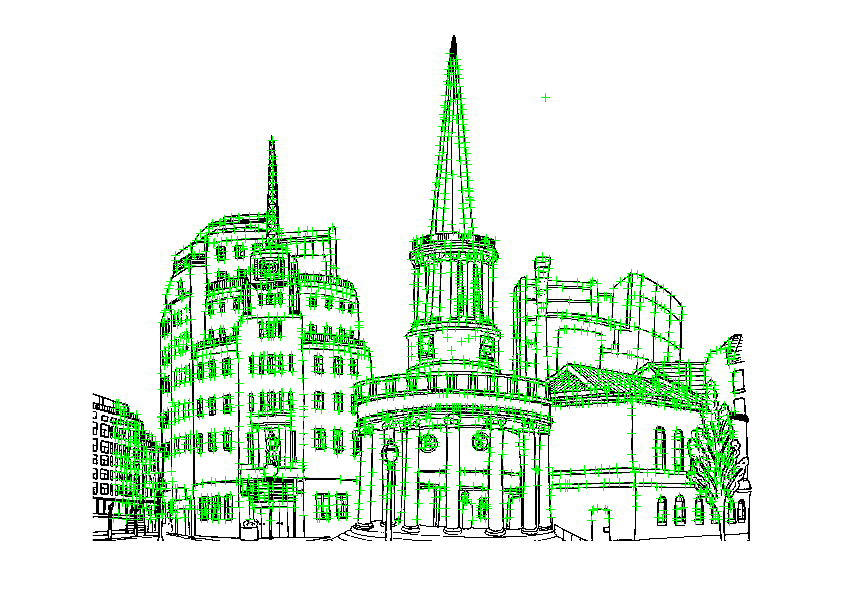
\includegraphics[scale=0.2]{pictures/all_souls_thresholded_interest_points}
	%        }
	%        \subfigure{
	%        \begin{tikzpicture}[font=\small]
    %            \begin{axis}[
    %                height=4cm,
    %                width=6cm,
    %                ybar,
    %                bar width=10pt,
    %                xlabel={Visual Words},
    %                ylabel={Counts},
    %                ymin=0,
    %                ytick=\empty,
    %                xtick=data,
    %                axis x line=bottom,
    %                axis y line=left,
    %                enlarge x limits=0.2,
    %                ylabel style={anchor=base,yshift=-1cm},
    %                symbolic x coords={1,2,3,4,5,6,7,8,...},
    %                axis lines=none,
    %            ]
    %                \addplot[fill=white] coordinates {
    %                    (1,5)
    %                    (2,10)
    %                    (3,50)
    %                    (4,20)
    %                    (5,15)
    %                    (6,4)
    %                    (7,40)
    %                    (8,1)
    %                    (...,0)
    %                };
    %            \end{axis}
    %        \end{tikzpicture}
    %        }
    %    \end{figure}
    %    
    %    \blfootnote{\url{http://dailydrawingdiary.com/wp-content/uploads/2012/05/bbc_all_souls_red_2s.jpg}}
	%\end{frame}
	
	\begin{frame}{\thesection.\thesubsection. Bag of Visual Words}
    	Intuition: assign local descriptors $y_{l,n}$ of image $x_n$ to visual words $\hat{y}_1,\ldots,\hat{y}_M$ previously obtained using clustering.
    	\vskip 0.5em

        \begin{figure}
            \centering
            \begin{tikzpicture}
                \begin{axis}[
                        axis equal image,
                        ticks=none,
                        height=6cm,
                        width=10cm,
                    ]
                    \addplot [only marks, black] table {pictures/points.txt};
                    \addplot [only marks, RWTHblue] (4.25,6);
                    \addplot [no markers, update limits=false] table {pictures/voronoi.txt};
                    \addplot [no markers, RWTHblue] coordinates {(4.25,6) (3,5)};
                    \node [below] at (axis cs:  4.9,  6.35) {{\color{RWTHblue} $y_{l,n}$}};
                    \node [below] at (axis cs:  3,  4.9) {$\hat{y}_m$};
                \end{axis}
            \end{tikzpicture}
    	\end{figure}
	\end{frame}
	
	\begin{frame}{\thesection.\thesubsection. Bag of Visual Words}
    	\begin{enumerate}[1.]
    	    \item Extract local descriptors $Y_n$ for each image $x_n$.
    	    \item Cluster all local descriptors $Y = \bigcup_{n = 1}^N Y_n$ to obtain visual words
        	    \begin{align*}
        	        \hat{Y} = \{\hat{y}_1, \ldots, \hat{y}_M\}.
        	    \end{align*}
        	\pause
    	    \item Assign each $y_{l,n} \in Y_n$ to nearest visual word (embedding step):
        	    \begin{align*}
			        f(y_{l,n}) = \left(\delta(\text{NN}_{\hat{Y}}(y_{l,n}) = \hat{y}_1),\ldots\right).
		        \end{align*}
		    \pause
		    \item Count visual word occurrences (aggregation step):
		        \begin{align*}
			        F(Y_n) = \sum_{l = 1}^L f(y_{l,n}).
		        \end{align*}
    	\end{enumerate}
    	\vskip 0.5em
	\end{frame}
	
	\subsection{Vector of Locally Aggregated Descriptors}
	\begin{frame}{\thesection.\thesubsection. Vector of Locally Aggregated Descriptors}
    	Intuition: consider the residuals $y_{l,n} - \hat{y}_m$ instead of counting visual words.
    	\vskip 0.5em

        \begin{figure}
            \centering
            \begin{tikzpicture}
                \begin{axis}[
                        axis equal image,
                        ticks=none,
                        height=6cm,
                        width=10cm,
                    ]
                    \addplot [only marks, black] table {pictures/points.txt};
                    \addplot [only marks, RWTHblue] (4,6);
                    \addplot [no markers, update limits=false] table {pictures/voronoi.txt};
                    \addplot [no markers, RWTHblue] coordinates {(4,6) (3,5)};
                    \node [below] at (axis cs:  4.65,  6.35) {{\color{RWTHblue} $y_{l,n}$}};
                    \node [below] at (axis cs:  3,  4.9) {$\hat{y}_m$};
                    \node [below] at (axis cs:  4.6,  5.75) {$\hat{y}_m - y_{l,n}$};
                \end{axis}
            \end{tikzpicture}
    	\end{figure}
	\end{frame}
	
	\begin{frame}{\thesection.\thesubsection. Vector of Locally Aggregated Descriptors}
	    \begin{enumerate}[1.]
	        \item Extract and cluster local descriptors.
	        \pause
	        \item Compute residuals of local descriptors visual words (embedding step):
	            \begin{align*}
	                f(y_{l,n}) = \left(\delta(\text{NN}_{\hat{Y}}(y_{l,n}) = \hat{y}_1)(y_{l,n} - \hat{y}_1),\ldots\right).
	            \end{align*}
	        \pause
	        \item Aggregate residuals (aggregation step):
	            \begin{align*}
			        F(Y_n) = \sum_{l = 1}^L f(y_{l,n}).
		        \end{align*}
		    \item $L_2$-normalize $F(Y_n)$ .
	    \end{enumerate}
	\end{frame}
	
	\subsection{Sparse-Coded Features}
	\begin{frame}{\thesection.\thesubsection. Sparse-Coded Features}
    	Intuition: soft-assign local descriptors to visual words.
    	\vskip 0.5em

        \begin{figure}
            \centering
            \begin{tikzpicture}
                \begin{axis}[
                        axis equal image,
                        ticks=none,
                        height=6cm,
                        width=10cm,
                    ]
                    \addplot [only marks, black] table {pictures/points.txt};
                    \addplot [only marks, RWTHblue] (3.2,6);
                    \addplot [no markers, update limits=false] table {pictures/voronoi.txt};
                    \addplot [no markers, RWTHblue] coordinates {(3.2,6) (3,5)};
                    \addplot [no markers, RWTHblue, opacity=0.75] coordinates {(3.2,6) (2,6)};
                    \node [below] at (axis cs:  3.85,  6.35) {{\color{RWTHblue} $y_{l,n}$}};
                    \node [below] at (axis cs:  3,  4.9) {$\hat{y}_m$};
                    \node [below] at (axis cs:  2,  6) {$\hat{y}_{m'}$};
                \end{axis}
            \end{tikzpicture}
    	\end{figure}
	\end{frame}
	
	\begin{frame}{\thesection.\thesubsection. Sparse-Coded Features}
	    \begin{enumerate}[1.]
	        \item Extract and cluster local descriptors.
	        \pause
	        \item Compute sparse codes (embedding step):
	            \begin{align*}
                    f(y_{l,n}) = \underset{r_l}{\text{arg} \text{min}} \|y_{l,n} - \hat{Y} r_l\|_2^2 + \lambda \| r_l \|_1.
                \end{align*}
                \begin{tikzpicture}[overlay,remember picture]
		            \draw[-latex new,arrow head=0.25cm,RWTHblue,shorten >=3pt,shorten <=3pt,thick,out=0,in=245] (3.5,0.25) node{\begin{tabular}{l}contains $\hat{y}_m$ as columns\end{tabular}} (5.5,0.25) to (6.4,0.85);
	            \end{tikzpicture}
	        \pause
	        \item Pool sparse codes (aggregation step):
	            \begin{align*}
	                F(Y_n) = \left(\max_{1 \leq l \leq L} \{f_1(y_{l,n})\}, \ldots\right)
	            \end{align*}
	            \begin{tikzpicture}[overlay,remember picture]
		            \draw[-latex new,arrow head=0.25cm,RWTHblue,shorten >=3pt,shorten <=3pt,thick,out=0,in=245] (3,0) node{\begin{tabular}{l}first component of $f(y_{l,n})$\end{tabular}} (5,0) to (6.25,0.75);
	            \end{tikzpicture}
	    \end{enumerate}
	\end{frame}
	
	\subsection{Compression and Nearest-Neighbor Search}
	\begin{frame}{\thesection.\thesubsection. Compression, Nearest-Neighbor Search}
	    Until now: image representation.
	    \vskip 0.5em
	    
	    Additional aspects of image retrieval:
	    \begin{itemize}
	        \item compression of image representations;
	        \item efficient indexing and nearest-neighbor search \cite{JegouDouzeSchmid:2011};
	        \item query expansion \cite{ChumPhilbinSivicIsardZisserman:2007} and spatial verification \cite{PhilbinChumIsardSivicZisserman:2007}.
	    \end{itemize}
	    \vskip 0.5em
	    \pause
	    
	    For example, compression can be accomplished using:
	    \begin{itemize}
	        \item Unsupervised methods, e.g. Principal Component Analysis (PCA);
	        \item or discriminate methods, e.g. Joint Subspace and Classifier Learning \cite{GordoSerranoPerronninValveny:2012} or Large Margin Dimensionality Reduction \cite{SimonyanParkhiVedaldiZisserman:2013}.
	    \end{itemize}
	    \begin{tikzpicture}[overlay,remember picture]
			\draw[-latex new,arrow head=0.25cm,RWTHblue,shorten >=3pt,shorten <=3pt,thick,out=195,in=295] (7.5,0) node{\begin{tabular}{l}discussed later ...\end{tabular}} (6,0) to (5,0.55);
		\end{tikzpicture}
	\end{frame}
	
	\section{Convolutional Neural Networks}	
	\subsection{Multi-layer Perceptrons}
	\begin{frame}{\thesection.\thesubsection. Multi-layer Perceptrons}
	    The prototypical neural network is the $L$-layer perceptron.
	    \vskip 0.5em
	    
	    Given input $x \in \mathbb{R}^{D}$, layer $l = 1$ computes for $1 \leq i \leq m^{(l)}$:
	    
	    \begin{figure}
	        \begin{tikzpicture}[shorten >=1pt]
				\tikzstyle{unit}=[draw,shape=circle,minimum size=1.15cm]
				%\tikzstyle{hidden}=[draw,shape=circle,fill=black!25,minimum size=1.15cm]
				\tikzstyle{hidden}=[draw,shape=circle,minimum size=1.15cm]

				%\node[unit](x0) at (-0.5,3.5){$y_1^{(l - 1)}$};
				\node[unit](x1) at (-0.5,2){$x_1$};
				\node at (-0.5,1){\vdots};
				\node[unit](xd) at (-0.5,-0.25){$x_D$};

				\node[hidden](h11) at (2.5,1){$y_i^{(1)}$};
                \node at (5.8,1){$= f\left(\sum_{j = 1}^{D} w_{i,j}^{(1)} x_j + w_{i,0}^{(1)}\right)$};
                
				%\draw[-latex new,arrow head=0.15cm] (x0) -- (h11);
				\draw[-latex new,arrow head=0.15cm] (x1) -- (h11);
				\draw[-latex new,arrow head=0.15cm] (xd) -- (h11);
			\end{tikzpicture}
	    \end{figure}
	    \begin{tikzpicture}[overlay,remember picture]
			\draw[-latex new,arrow head=0.25cm,RWTHblue,shorten >=3pt,shorten <=3pt,thick,out=195,in=295] (9,1.75) node{\begin{tabular}{l}e.g. $f(z) = \frac{1}{1 + \exp(-z)}$\end{tabular}} (7.2,1.75) to (6.4,2.55);
		\end{tikzpicture}
	\end{frame}
	
	\begin{frame}{\thesection.\thesubsection. Multi-layer Perceptrons}
	    The prototypical neural network is the $L$-layer perceptron.
	    \vskip 0.5em
	    
	    Given input $y^{(0)} := x \in \mathbb{R}^{m^{(0)}}$, layer $l$ computes for $1 \leq i \leq m^{(l)}$:
	    
	    \begin{figure}
	        \begin{tikzpicture}[shorten >=1pt]
				\tikzstyle{unit}=[draw,shape=circle,minimum size=1.15cm]
				%\tikzstyle{hidden}=[draw,shape=circle,fill=black!25,minimum size=1.15cm]
				\tikzstyle{hidden}=[draw,shape=circle,minimum size=1.15cm]

				%\node[unit](x0) at (-0.5,3.5){$y_1^{(l - 1)}$};
				\node[unit](x1) at (-0.5,2){$y_1^{(l - 1)}$};
				\node at (-0.5,1){\vdots};
				\node[unit](xd) at (-0.5,-0.25){$y_{m^{(l - 1)}}^{(l - 1)}$};

				\node[hidden](h11) at (2.5,1){$y_i^{(l)}$};
                \node at (5.8,1){$= f\left(\sum_{j = 1}^{m^{(l - 1)}} w_{i,j}^{(l)} y_j^{(l - 1)} + w_{i,0}^{(l)}\right)$};
                
				%\draw[-latex new,arrow head=0.15cm] (x0) -- (h11);
				\draw[-latex new,arrow head=0.15cm] (x1) -- (h11);
				\draw[-latex new,arrow head=0.15cm] (xd) -- (h11);
			\end{tikzpicture}
	    \end{figure}
	    \begin{tikzpicture}[overlay,remember picture]
			\draw[-latex new,arrow head=0.25cm,RWTHblue,shorten >=3pt,shorten <=3pt,thick,out=195,in=295] (9,1.75) node{\begin{tabular}{l}e.g. $f(z) = \frac{1}{1 + \exp(-z)}$\end{tabular}} (7.2,1.75) to (5.9,2.75);
		\end{tikzpicture}
	\end{frame}
	
	\begin{frame}{\thesection.\thesubsection. Multi-layer Perceptrons}
	    \begin{figure}[t]
			\centering
			\begin{tikzpicture}[shorten >=1pt]
				\tikzstyle{unit}=[draw,shape=circle,minimum size=1.15cm]
				%\tikzstyle{hidden}=[draw,shape=circle,fill=black!25,minimum size=1.15cm]
				\tikzstyle{hidden}=[draw,shape=circle,minimum size=1.15cm]

				\node[unit](x0) at (-0.5,3.5){$x_1$};
				\node[unit](x1) at (-0.5,2){$x_2$};
				\node at (-0.5,1){\vdots};
				\node[unit](xd) at (-0.5,0){$x_D$};

				\node[hidden](h10) at (2.5,4){$y_1^{(1)}$};
				\node[hidden](h11) at (2.5,2.5){$y_2^{(1)}$};
				\node at (2.5,1.5){\vdots};
				\node[hidden](h1m) at (2.5,-0.5){$y_{m^{(1)}}^{(1)}$};

				\node(h22) at (4.25,1){};
				\node(h21) at (4.25,3){};
		
				\node(d2) at (4.5,1){$\ldots$};
				\node(d1) at (4.5,3){$\ldots$};

				\node(hL12) at (4.75,1){};
				\node(hL11) at (4.75,3){};

				\node[hidden](hL0) at (6.5,4.25){$y_1^{(L-1)}$};
				\node[hidden](hL1) at (6.5,2.5){$y_2^{(L-1)}$};
				\node at (6.5,1.5){\vdots};
				\node[hidden](hLm) at (6.5,-0.5){$y_{m^{(L-1)}}^{(L-1)}$};

				\node[unit](y1) at (9.5,3.75){$y_1^{(L)}$};
				\node[unit](y2) at (9.5,2){$y_2^{(L)}$};
				\node at (9.5,1){\vdots};	
				\node[unit](yc) at (9.5,-0.25){$y_{m^{(L)}}^{(L)}$};

				\draw[-latex new,arrow head=0.15cm] (x0) -- (h10);
				\draw[-latex new,arrow head=0.15cm] (x0) -- (h11);
				\draw[-latex new,arrow head=0.15cm] (x0) -- (h1m);

				\draw[-latex new,arrow head=0.15cm] (x1) -- (h10);
				\draw[-latex new,arrow head=0.15cm] (x1) -- (h11);
				\draw[-latex new,arrow head=0.15cm] (x1) -- (h1m);

				\draw[-latex new,arrow head=0.15cm] (xd) -- (h10);
				\draw[-latex new,arrow head=0.15cm] (xd) -- (h11);
				\draw[-latex new,arrow head=0.15cm] (xd) -- (h1m);

				\draw[-latex new,arrow head=0.15cm] (hL0) -- (y1);
				\draw[-latex new,arrow head=0.15cm] (hL0) -- (yc);
				\draw[-latex new,arrow head=0.15cm] (hL0) -- (y2);

				\draw[-latex new,arrow head=0.15cm] (hL1) -- (y1);
				\draw[-latex new,arrow head=0.15cm] (hL1) -- (yc);
				\draw[-latex new,arrow head=0.15cm] (hL1) -- (y2);

				\draw[-latex new,arrow head=0.15cm] (hLm) -- (y1);
				\draw[-latex new,arrow head=0.15cm] (hLm) -- (y2);
				\draw[-latex new,arrow head=0.15cm] (hLm) -- (yc);

				\draw[-latex new,arrow head=0.15cm,path fading=east] (h10) -- (h21);
				\draw[-latex new,arrow head=0.15cm,path fading=east] (h10) -- (h22);
		
				\draw[-latex new,arrow head=0.15cm,path fading=east] (h11) -- (h21);
				\draw[-latex new,arrow head=0.15cm,path fading=east] (h11) -- (h22);
		
				\draw[-latex new,arrow head=0.15cm,path fading=east] (h1m) -- (h21);
				\draw[-latex new,arrow head=0.15cm,path fading=east] (h1m) -- (h22);
		
				\draw[-latex new,arrow head=0.15cm,path fading=west] (hL11) -- (hL0);
				\draw[-latex new,arrow head=0.15cm,path fading=west] (hL12) -- (hL0);
		
				\draw[-latex new,arrow head=0.15cm,path fading=west] (hL11) -- (hL1);
				\draw[-latex new,arrow head=0.15cm,path fading=west] (hL12) -- (hL1);
		
				\draw[-latex new,arrow head=0.15cm,path fading=west] (hL11) -- (hLm);
				\draw[-latex new,arrow head=0.15cm,path fading=west] (hL12) -- (hLm);
		
				\draw [decorate,decoration={brace,amplitude=10pt},xshift=-4pt,yshift=0pt] (-1,4) -- (0.25,4) node [black,midway,yshift=+0.6cm]{input};
				\draw [decorate,decoration={brace,amplitude=10pt},xshift=-4pt,yshift=0pt] (2,4.5) -- (3.25,4.5) node [black,midway,yshift=+0.6cm]{$1^{\text{st}}$ layer};
				\draw [decorate,decoration={brace,amplitude=10pt},xshift=-4pt,yshift=0pt] (6,5) -- (7.25,5) node [black,midway,yshift=+0.6cm]{$(L-1)^{\text{th}}$ layer};
				\draw [decorate,decoration={brace,amplitude=10pt},xshift=-4pt,yshift=0pt] (9,4.25) -- (10.25,4.25) node [black,midway,yshift=+0.6cm]{output};
			\end{tikzpicture}
			\label{fig:multilayer-perceptron}
		\end{figure}
	\end{frame}
	
	%\begin{frame}{Neural Networks in $\not{3}$ \sout{$2$} 1 Slide(s)}
	%    Classification using $L$-layer perceptrons: use the softmax activation function
	%    \begin{tikzpicture}[overlay,remember picture]
	%		\draw[-latex new,arrow head=0.25cm,RWTHblue,shorten >=3pt,shorten <=3pt,thick,out=45,in=120] (0.25,-0.75) node{\begin{tabular}{l}interpreted as\\posterior probabilities\end{tabular}} (1,-0.75) to (2.5,-0.85);
	%	\end{tikzpicture}
	%    \begin{align*}
	%        f(z_i^{(L)}) = \frac{\exp\left(z_i^{(l)}\right)}{\sum_{j = 1}^{m^{(L)}} \exp\left(z_j^{(L)}\right)}
	%    \end{align*}
	%    in the last (i.e. $l = L$) layer.
	%    \vskip 0.5em
	%    
	%    Given a training set $\{(x_n, t_n)\}$ with $t_n = i$ iff $x_n$ belongs to class $i$, choose an loss function such as the multinomial loss
	%    \begin{tikzpicture}[overlay,remember picture]
	%		\draw[-latex new,arrow head=0.25cm,RWTHblue,shorten >=3pt,shorten <=3pt,thick,out=45,in=120] (-7,-1) node{\begin{tabular}{l}all weights\\of the network\end{tabular}} (-6.25,-1) to (-4.5,-0.75);
	%	\end{tikzpicture}
	%    \begin{align*}
	%        E(W) = - \frac{1}{m^{(L)}} \sum_{n = 1}^N \log\left(y_{t_n}^{(L)}\right)
	%    \end{align*}
	%    and minimize it using gradient methods.
	%\end{frame}
	
	\subsection{Convolutional Neural Networks}
	\begin{frame}{\thesection.\thesubsection. Convolutional Neural Networks}
	    Motivation:
	    \begin{itemize}
	        \item Multi-layer perceptrons do not naturally accept images as input;
	        \item however, spatial information is important.
	    \end{itemize}
	    \vskip 0.5em
	    \pause
	    
	    Solution: convolutional neural networks.
	    \vskip 0.5em
	    
	    Intuition: apply learned filters on the input image to compute a set of feature maps.
	    \vskip 0.5em
	    
	    Repeat: normalize and pool feature maps before applying another set of learned filters.
	    \vskip 0.5em
	    
	    Apply a multi-layer perceptron on the obtained (small) feature maps.
	\end{frame}

    \begin{frame}{\thesection.\thesubsection. Convolutional Layer}
	    General architecture:
	    \begin{center}
	        \textbf{convolutional layer} -- contrast normalization layer -- pooling layer
	    \end{center}
	    
	    \begin{figure}
	        \begin{tikzpicture}[scale=0.7]
		        \node at (1.5,4.75){\begin{tabular}{c}input image\end{tabular}};
	
		        \draw (0,0) -- (3,0) -- (3,3) -- (0,3) -- (0,0);
		
		        \draw (2,2) -- (2.5,2) -- (2.5,2.5) -- (2,2.5) -- (2,2);
		        \draw (2,0.5) -- (2.5,0.5) -- (2.5,1) -- (2,1) -- (2,0.5);
		        \draw (1,1) -- (1.5,1) -- (1.5,1.5) -- (1,1.5) -- (1,1);
		
		        \draw (2.5,2) -- (7,3.25);
		        \draw (2.5,2.5) -- (7,3.25);

		        \draw (2.5,1) -- (5.75,0.25);
		        \draw (2.5,0.5) -- (5.75,0.25);
		
		        \draw (1.5,1.5) -- (5.5,1.25);
		        \draw (1.5,1) -- (5.5,1.25);
		
		        \node at (5.75,4.75){\begin{tabular}{c}feature maps\\layer $l = 1$\end{tabular}};
		
		        \draw[fill=black,opacity=0.2,draw=black] (5.5,1.5) -- (7.5,1.5) -- (7.5,3.5) -- (5.5,3.5) -- (5.5,1.5);
		        \draw[fill=black,opacity=0.2,draw=black] (5,1) -- (7,1) -- (7,3) -- (5,3) -- (5,1);
		        \draw[fill=black,opacity=0.2,draw=black] (4.5,0.5) -- (6.5,0.5) -- (6.5,2.5) -- (4.5,2.5) -- (4.5,0.5);
		        \draw[fill=black,opacity=0.2,draw=black] (4,0) -- (6,0) -- (6,2) -- (4,2) -- (4,0);
	        \end{tikzpicture}
	    \end{figure}
	\end{frame}
	
	\begin{frame}{\thesection.\thesubsection. Convolutional Layer}
	    General architecture:
	    \begin{center}
	        \textbf{convolutional layer} -- contrast normalization layer -- pooling layer
	    \end{center}
	    
	    \begin{figure}
	        \begin{tikzpicture}[scale=0.7]
		        \node at (1.5,4.75){\begin{tabular}{c}feature map\\layer $(l - 1)$\end{tabular}};
	
		        \draw (0,0) -- (3,0) -- (3,3) -- (0,3) -- (0,0);
		
		        \draw (2,2) -- (2.5,2) -- (2.5,2.5) -- (2,2.5) -- (2,2);
		        \draw (2,0.5) -- (2.5,0.5) -- (2.5,1) -- (2,1) -- (2,0.5);
		        \draw (1,1) -- (1.5,1) -- (1.5,1.5) -- (1,1.5) -- (1,1);
		
		        \draw (2.5,2) -- (7,3.25);
		        \draw (2.5,2.5) -- (7,3.25);

		        \draw (2.5,1) -- (5.75,0.25);
		        \draw (2.5,0.5) -- (5.75,0.25);
		
		        \draw (1.5,1.5) -- (5.5,1.25);
		        \draw (1.5,1) -- (5.5,1.25);
		
		        \node at (5.75,4.75){\begin{tabular}{c}feature maps\\layer $l$\end{tabular}};
		
		        \draw[fill=black,opacity=0.2,draw=black] (5.5,1.5) -- (7.5,1.5) -- (7.5,3.5) -- (5.5,3.5) -- (5.5,1.5);
		        \draw[fill=black,opacity=0.2,draw=black] (5,1) -- (7,1) -- (7,3) -- (5,3) -- (5,1);
		        \draw[fill=black,opacity=0.2,draw=black] (4.5,0.5) -- (6.5,0.5) -- (6.5,2.5) -- (4.5,2.5) -- (4.5,0.5);
		        \draw[fill=black,opacity=0.2,draw=black] (4,0) -- (6,0) -- (6,2) -- (4,2) -- (4,0);
	        \end{tikzpicture}
	    \end{figure}
	\end{frame}
	
	\begin{frame}{\thesection.\thesubsection. Convolutional Layer}
	    General architecture:
	    \begin{center}
	        \textbf{convolutional layer} -- contrast normalization layer -- pooling layer
	    \end{center}
	    \vskip 0.5em
	    
	    Given $m_1^{(l - 1)}$ feature maps $Y_j^{(l - 1)}$, layer $l$ computes
	    \begin{tikzpicture}[overlay,remember picture]
		%	\draw[-latex new,arrow head=0.25cm,RWTHblue,shorten >=3pt,shorten <=3pt,thick,out=180,in=80] (-5,-0.4) node{\begin{tabular}{l}layer $l$\end{tabular}} (-5.5,-0.4) to (-6.6,-1.25);
		%	\draw[-latex new,arrow head=0.25cm,RWTHblue,shorten >=3pt,shorten <=3pt,thick,out=170,in=285] (-4.5,-2.6) node{\begin{tabular}{l}feature map $i$\end{tabular}} (-5.75,-2.5) to (-6.85,-1.8);
		    \draw[-latex new,arrow head=0.25cm,RWTHblue,shorten >=3pt,shorten <=3pt,thick,out=170,in=270] (0.15,-2.5) node{\begin{tabular}{l}discrete convolution\end{tabular}} (-1.5,-2.5) to (-2.25,-1.6);
		\end{tikzpicture}
	    \begin{align*}
	        Y_i^{(l)} = f\left(B_i^{(l)} + \sum_{j = 1}^{m_1^{(l - 1)}} W_{i,j}^{(l)} \ast Y_j^{(l - 1)}\right),\quad 1 \leq i \leq m_1^{(l)}\label{eq:convolutional-layer}
	    \end{align*}
	    \vspace{0.5em}
	    where $B_i^{(1)}$ are bias matrices and $W_{i,j}^{(1)}$ are filters.
	\end{frame}
	
	\begin{frame}{\thesection.\thesubsection. Local Contrast Normalization Layer}
	    General architecture:
	    \begin{center}
	        convolutional layer -- \textbf{contrast normalization layer} -- pooling layer
	    \end{center}
	    \vskip 0.5em
	    
	    \begin{figure}
	        \begin{tikzpicture}[scale=0.9]
	            \node at (1.75,4.25){\begin{tabular}{c}feature maps\\layer $(l - 1)$\end{tabular}};
	            
			    \draw[fill=black,opacity=0.2,draw=black] (1,1) -- (3,1) -- (3,3) -- (1,3) -- (1,1);
			    \draw[fill=black,opacity=0.2,draw=black] (0.5,0.5) -- (2.5,0.5) -- (2.5,2.5) -- (0.5,2.5) -- (0.5,0.5);
			    \draw[fill=black,opacity=0.2,draw=black] (0,0) -- (2,0) -- (2,2) -- (0,2) -- (0,0);
			
			    \draw[opacity=0.4,draw=red,fill=red] (2.3,2.25) -- (2.75,2.3) -- (2.75,2.75) -- (2.3,2.75) -- (2.3,2.3);
			    \draw[opacity=0.4,draw=red,fill=red] (1.8,1.8) -- (2.25,1.8) -- (2.25,2.25) -- (1.8,2.25) -- (1.8,1.8);
			    \draw[opacity=0.4,draw=red,fill=red] (1.3,1.3) -- (1.75,1.3) -- (1.75,1.75) -- (1.3,1.75) -- (1.3,1.3);
			    \draw[opacity=0.4,draw=red](1.3,1.75) --  (1.8,2.25);
			    \draw[opacity=0.4,draw=red](1.75,1.3) -- (2.25,1.8);
			    \draw[opacity=0.4,draw=red](2.25,1.8) -- (2.75,2.3);
			    \draw[opacity=0.4,draw=red](1.8,2.25) -- (2.3,2.75);
			
			    \node at (6,1.5){\begin{tabular}{l}ensure that values\\are comparable\end{tabular}};
		    \end{tikzpicture}
	    \end{figure}
	\end{frame}
	
	\begin{frame}{\thesection.\thesubsection. Local Contrast Normalization Layer}
        General architecture:
        \begin{center}
            convolutional layer -- \textbf{contrast normalization layer} -- pooling layer
        \end{center}
        \vskip 0.5em
        
        Given $m_1^{(l - 1)}$ feature maps $Y_j^{(l - 1)}$, brightness normalization \cite{KrizhevskySutskeverHinton:2012} computes
        \begin{align*}
            \left(Y_i^{(l)}\right)_{r,s} = \frac{\left(Y_i^{(l - 1)}\right)_{r,s}}{1 + \sum_{j = 1}^{m_1^{(l - 1)}} \left(Y_j^{(l - 1)}\right)_{r,s}^2},\quad 1 \leq i \leq m_1^{(l)} = m_1^{(l - 1)}.
        \end{align*}
        %\begin{tikzpicture}[overlay,remember picture]
		%    \draw[-latex new,arrow head=0.25cm,RWTHblue,shorten >=3pt,shorten <=3pt,thick,out=180,in=290] (6.5,0) node{\begin{tabular}{l}``adjacent'' feature maps\end{tabular}} (4.5,0) to (3.5,0.5);
	    %\end{tikzpicture}
    \end{frame}
	
	\begin{frame}{\thesection.\thesubsection. Pooling Layer}
	    General architecture:
	    \begin{center}
	        convolutional layer -- contrast normalization layer -- \textbf{pooling layer}
	    \end{center}
	    \vskip 0.5em
	    
	    \begin{figure}
	        \begin{tikzpicture}[scale=0.7]
		        \node at (1.75,4.75){\begin{tabular}{c}feature maps\\layer $(l-1)$\end{tabular}};
		
		        \draw[fill=black,opacity=0.2,draw=black] (1.5,1.5) -- (3.5,1.5) -- (3.5,3.5) -- (1.5,3.5) -- (1.5,1.5);
		        \draw[fill=black,opacity=0.2,draw=black] (1,1) -- (3,1) -- (3,3) -- (1,3) -- (1,1);
		        \draw[fill=black,opacity=0.2,draw=black] (0.5,0.5) -- (2.5,0.5) -- (2.5,2.5) -- (0.5,2.5) -- (0.5,0.5);
		        \draw[fill=black,opacity=0.2,draw=black] (0,0) -- (2,0) -- (2,2) -- (0,2) -- (0,0);
		
		        \draw (3.1,3.1) -- (3.4,3.1) -- (3.4,3.4) -- (3.1,3.4) -- (3.1,3.1);
		        \draw (2.6,1.1) -- (2.9,1.1) -- (2.9,1.4) -- (2.6,1.4) -- (2.6,1.1);
		        \draw (1.1,0.1) -- (1.4,0.1) -- (1.4,0.4) -- (1.1,0.4) -- (1.1,0.1);
		
		        \draw (3.4,3.4) -- (7.8,2.8);
		        \draw (3.4,3.1) -- (7.8,2.8);
		
		        \draw (2.9,1.4) -- (7.3,1.2);
		        \draw (2.9,1.1) -- (7.3,1.2);
		
		        \draw (1.4,0.4) -- (5.9,0.3);
		        \draw (1.4,0.1) -- (5.9,0.3);
		
		        \node at (6.5,4.75){\begin{tabular}{c}feature maps\\layer $l$\end{tabular}};
		
		        \draw[fill=black,opacity=0.2,draw=black] (6.5,1.5) -- (8,1.5) -- (8,3) -- (6.5,3) -- (6.5,1.5);
		        \draw[fill=black,opacity=0.2,draw=black] (6,1) -- (7.5,1) -- (7.5,2.5) -- (6,2.5) -- (6,1);
		        \draw[fill=black,opacity=0.2,draw=black] (5.5,0.5) -- (7,0.5) -- (7,2) -- (5.5,2) -- (5.5,0.5);
		        \draw[fill=black,opacity=0.2,draw=black] (5,0) -- (6.5,0) -- (6.5,1.5) -- (5,1.5) -- (5,0);
	        \end{tikzpicture}
	    \end{figure}
	\end{frame}
	
	\begin{frame}{\thesection.\thesubsection. Pooling Layer}
        General architecture:
        \begin{center}
            convolutional layer -- contrast normalization layer -- \textbf{pooling layer}
        \end{center}
        \vskip 0.5em
        
        Given feature maps $Y_j^{(l - 1)}$ of size $m_2^{(l - 1)} \times m_3^{(l - 1)}$, it computes feature maps $Y_i^{(l)}$ of reduced size by
        \begin{itemize}
            \item computing the average value within (non-overlapping) windows (average pooling);
            \item or keeping the maximum value of (non-overlapping) windows (max pooling).
        \end{itemize}
    \end{frame}
	
	\subsection{Architectures}
	\begin{frame}{\thesection.\thesubsection. Schematic Architecture}
	    \begin{figure}
			\centering
			\begin{tikzpicture}
				\node at (0.5,-0.75){\begin{tabular}{c}input image\end{tabular}};
		
				\draw (0,0) -- (1,0) -- (1,1) -- (0,1) -- (0,0);
		
				\node at (3,3){\begin{tabular}{c}convolutional layer\end{tabular}};
		
				\draw[fill=black,opacity=0.2,draw=black] (2.75,1.25) -- (3.75,1.25) -- (3.75,2.25) -- (2.75,2.25) -- (2.75,1.25);
				\draw[fill=black,opacity=0.2,draw=black] (2.5,1) -- (3.5,1) -- (3.5,2) -- (2.5,2) -- (2.5,1);
				\draw[fill=black,opacity=0.2,draw=black] (2.25,0.75) -- (3.25,0.75) -- (3.25,1.75) -- (2.25,1.75) -- (2.25,0.75);
				\draw[fill=black,opacity=0.2,draw=black] (2,0.5) -- (3,0.5) -- (3,1.5) -- (2,1.5) -- (2,0.5);
				\draw[fill=black,opacity=0.2,draw=black] (1.75,0.25) -- (2.75,0.25) -- (2.75,1.25) -- (1.75,1.25) -- (1.75,0.25);
				\draw[fill=black,opacity=0.2,draw=black] (1.5,0) -- (2.5,0) -- (2.5,1) -- (1.5,1) -- (1.5,0);
		
				\node at (4.5,-0.75){\begin{tabular}{c}pooling layer\end{tabular}};
		
				\draw[fill=black,opacity=0.2,draw=black] (5,1.25) -- (5.75,1.25) -- (5.75,2) -- (5,2) -- (5,1.25);
				\draw[fill=black,opacity=0.2,draw=black] (4.75,1) -- (5.5,1) -- (5.5,1.75) -- (4.75,1.75) -- (4.75,1);
				\draw[fill=black,opacity=0.2,draw=black] (4.5,0.75) -- (5.25,0.75) -- (5.25,1.5) -- (4.5,1.5) -- (4.5,0.75);
				\draw[fill=black,opacity=0.2,draw=black] (4.25,0.5) -- (5,0.5) -- (5,1.25) -- (4.25,1.25) -- (4.25,0.5);
				\draw[fill=black,opacity=0.2,draw=black] (4,0.25) -- (4.75,0.25) -- (4.75,1) -- (4,1) -- (4,0.25);
				\draw[fill=black,opacity=0.2,draw=black] (3.75,0) -- (4.5,0) -- (4.5,0.75) -- (3.75,0.75) -- (3.75,0);
		
				\node at (6.5,1){$\ldots$};
				\node at (8.5,3){\begin{tabular}{c}two-layer perceptron\end{tabular}};
		
				\draw[fill=black,draw=black,opacity=0.5] (6.5,0) -- (7,0) -- (8.5,1.75) -- (8,1.75) -- (6.5,0);
				\draw[fill=black,draw=black,opacity=0.5] (8.5,0.5) -- (9,0.5) -- (9.65,1.25) -- (9.15,1.25) -- (8.5,0.5);
			\end{tikzpicture}
			\label{fig:traditional-convolutional-network}
		\end{figure}
	\end{frame}
	
	\begin{frame}{\thesection.\thesubsection. ImageNet Architecture ``AlexNet''}
		\begin{figure}
			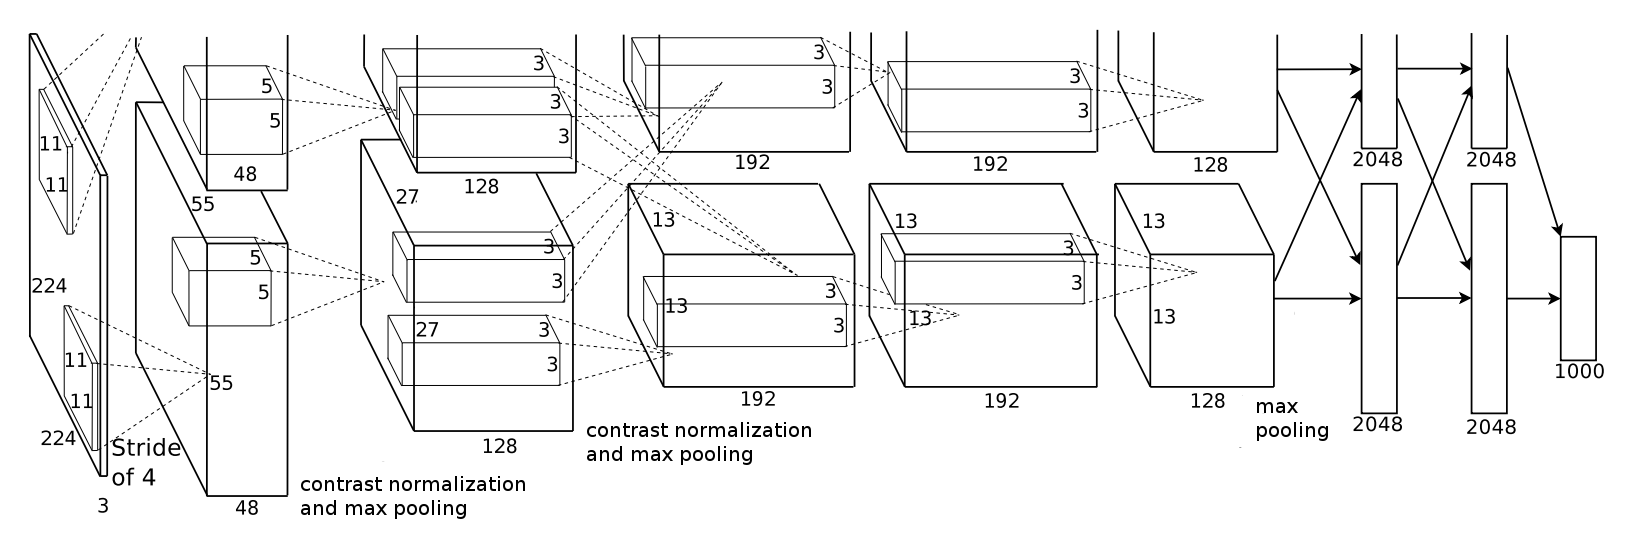
\includegraphics[scale=0.35]{pictures/architecture}
			\caption{Architecture used by Krizhevsky et al. \cite{KrizhevskySutskeverHinton:2012}, $L = 13$.}
		\end{figure}
	\end{frame}
	
	\subsection{Training}
	\begin{frame}{\thesection.\thesubsection. Training}
	    For classification, use softmax activation function in layer $L$:
	    \begin{align*}
	        f(z_i^{(L)}) = \frac{\exp\left(z_i^{(L)}\right)}{\sum_{j = 1}^{m^{(L)}} \exp\left(z_j^{(L)}\right)}.
	    \end{align*}
	    \begin{tikzpicture}[overlay,remember picture]
			\draw[-latex new,arrow head=0.25cm,RWTHblue,shorten >=3pt,shorten <=3pt,thick,out=45,in=135] (2,1) node{\begin{tabular}{l}interpreted as\\posteriors\end{tabular}} (2,1.5) to (4,1.5);
		\end{tikzpicture}
	    \vskip 0.5em
	    \pause
	    
	    Given a training set $\{(x_n, t_n)\}$ with $t_n = i$ iff $x_n$ belongs to class $i$, minimize multinomial loss
	    \begin{tikzpicture}[overlay,remember picture]
			\draw[-latex new,arrow head=0.25cm,RWTHblue,shorten >=3pt,shorten <=3pt,thick,out=45,in=120] (-2.5,-1) node{\begin{tabular}{l}all weights\\of the network\end{tabular}} (-1.75,-1) to (-0.15,-0.8);
		\end{tikzpicture}
	    \begin{align*}
	        E(W) = - \frac{1}{m^{(L)}} \sum_{n = 1}^N \log\left(y_{t_n}^{(L)}\right)
	    \end{align*}
	    using gradient descent.
	\end{frame}
	
	\section{Neural Codes for Image Retrieval}
	\begin{frame}{\thesection. Neural Codes -- Motivation}
	    \begin{figure}
	        \subfigure{
	            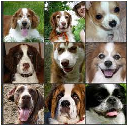
\includegraphics[scale=1]{pictures/layer-4}
	        }
	        \subfigure{
	            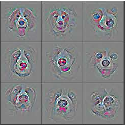
\includegraphics[scale=1]{pictures/layer-4-activations}
	        }
	        \caption{Back-projection of a single feature activation in the fourth convolutional layer \cite{ZeilerFergus:2014}.}
	    \end{figure}
	\end{frame}
	
	\begin{frame}{\thesection. Neural Codes for Image Retrieval}
        Motivation: Intermediate feature activations are rich representations of image content.
        \vskip 0.5em
        
        For application in image retrieval, Babenko et al. \cite{BabenkoSlesarevChigorinLempitsky:2014} use
        \begin{itemize}
            \item layer $l = 10$: last convolutional layer, including subsequent max pooling;
            \item layer $l = 11$ and $l = 12$: first and second layer of the three-layer perceptron.
        \end{itemize}
        \vskip 0.5em
        \pause
        
        Two models:
        \begin{itemize}
            \item pre-trained on ImageNet\footnote{Available at \url{http://www.image-net.org/}.} ($\sim3.2$ million images, $>1000$ classes);
            \item and re-trained on the Landmark dataset ($213,678$ images of $672$ popular landmarks).
        \end{itemize}
	\end{frame}
	
	\begin{frame}{\thesection. Neural Codes for Image Retrieval}
	    \begin{figure}
		    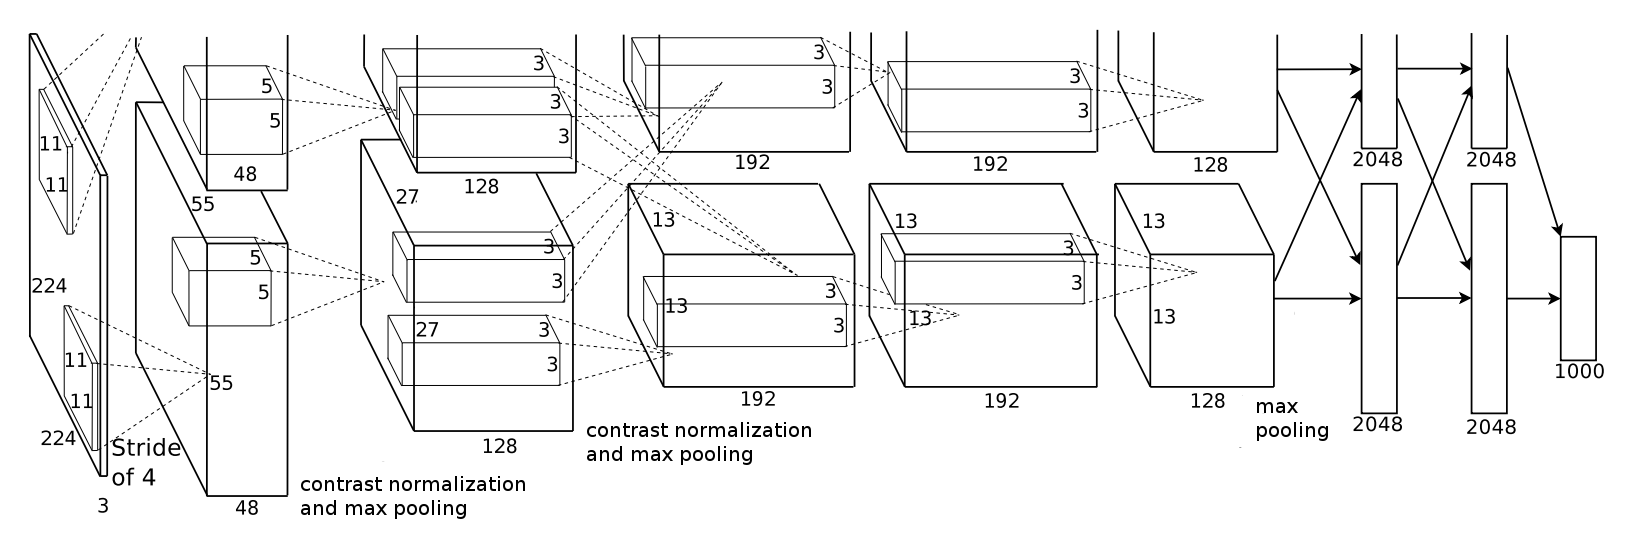
\includegraphics[scale=0.35]{pictures/architecture}
		    \begin{tikzpicture}[overlay,remember picture]
		        \draw[-latex new,arrow head=0.25cm,RWTHblue,shorten >=3pt,shorten <=3pt,thick,out=0,in=250] (-4.25,0) node{\begin{tabular}{l}layer $l = 10$\end{tabular}} (-3.25,0) to (-2.5,0.75);
		        \draw[-latex new,arrow head=0.25cm,RWTHblue,shorten >=3pt,shorten <=3pt,thick,out=0,in=250] (-3.75,-0.5) node{\begin{tabular}{l}layer $l = 11$\end{tabular}} (-2.75,-0.5) to (-1.85,0.8);
		        \draw[-latex new,arrow head=0.25cm,RWTHblue,shorten >=3pt,shorten <=3pt,thick,out=0,in=105] (-3.5,4.5) node{\begin{tabular}{l}layer $l = 12$\end{tabular}} (-2.5,4.5) to (-1.1,3.85);
	        \end{tikzpicture}
	          \vskip 1em
		    \caption{Architecture used by Krizhevsky et al. \cite{KrizhevskySutskeverHinton:2012}, $L = 13$.}
	    \end{figure}
	\end{frame}
	
	\begin{frame}{\thesection. Compressed Neural Codes}
	    Compression using PCA and Large Margin Dimensionality Reduction.
	    \vskip 0.5em
        \pause
        
        Large Margin Dimensionality Reduction:
        \begin{enumerate}[1.]
            \item Match images such that $t_{n,n'} = 1$ iff images $x_n$ and $x_{n'}$ are related.
            \item Compute linear dimensionality reduction $P \in \mathbb{R}^{C' \times C}$ by minimizing
                \begin{align*}
	                E(P) = \sum_{n,n'}^N \max\{0, \textcolor{black}{1 - t_{n,n'}\left(b - (x_n - x_{n'})^T P^T P (x_n - x_{n'})\right)}\}
	            \end{align*}
	            \begin{tikzpicture}[overlay,remember picture]
		            \draw[-latex new,arrow head=0.25cm,RWTHblue,shorten >=3pt,shorten <=3pt,thick,out=180,in=280] (9.25,0.5) node{\begin{tabular}{l}large margin condition\end{tabular}} (7.5,0.5) to (7,1.15);
	            \end{tikzpicture}
	            using gradient descent.
        \end{enumerate}
	\end{frame}
	
	\section{Experiments}
	\begin{frame}{\thesection. Datasets and Metric}
	    \only<1>{
	        Datasets:
	        \begin{itemize}
	            \item \textbf{Oxford 5k} \cite{PhilbinChumIsardSivicZisserman:2007}: $5,062$ images of eleven different landmarks in Oxford; $5$ queries with ground truth per landmark.
	            \item INRIA Holidays \cite{JegouDouzeSchmid:2008}: $1,491$ holiday images with $500$ distinct queries including ground truth.
	        \end{itemize}
	        \vskip 0.5em
	        
	        \begin{figure}
	            \centering
	            \subfigure{
	                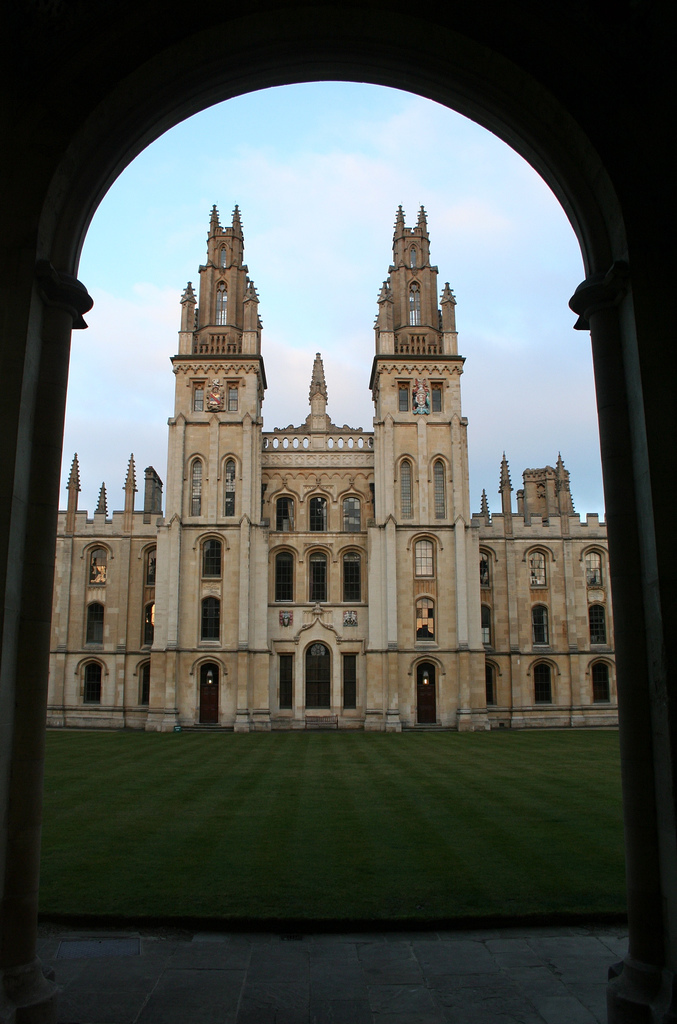
\includegraphics[scale=0.075]{pictures/all_souls_000002}
	            }
	            \subfigure{
	                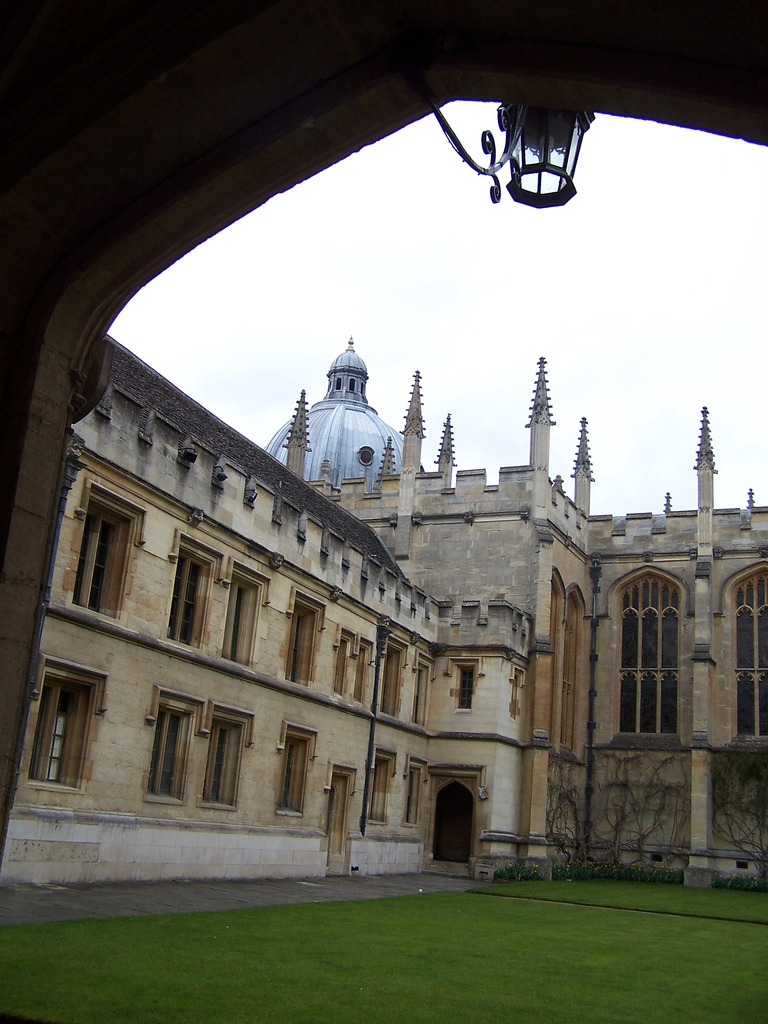
\includegraphics[scale=0.075]{pictures/all_souls_000007}
	            }
	            \subfigure{
	                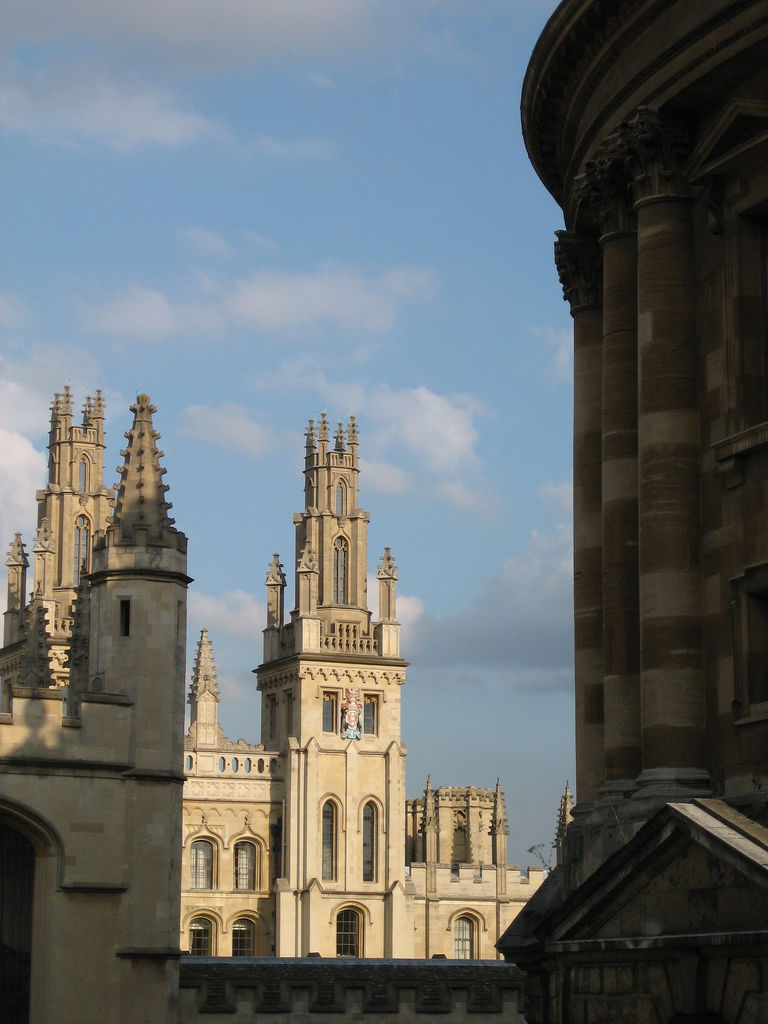
\includegraphics[scale=0.075]{pictures/all_souls_000063}
	            }
	            \caption{Example images from the Oxford 5k dataset showing the All Souls College of the University of Oxford.}
	        \end{figure}
	    }
	    \only<2>{
	        Datasets:
	        \begin{itemize}
	            \item Oxford 5k \cite{PhilbinChumIsardSivicZisserman:2007}: $5,062$ images of eleven different landmarks in Oxford; $5$ queries with ground truth per landmark.
	            \item \textbf{INRIA Holidays} \cite{JegouDouzeSchmid:2008}: $1,491$ holiday images with $500$ distinct queries including ground truth.
	        \end{itemize}
	        \vskip 0.5em
	        
	        \begin{figure}
	            \centering
	            \subfigure{
	                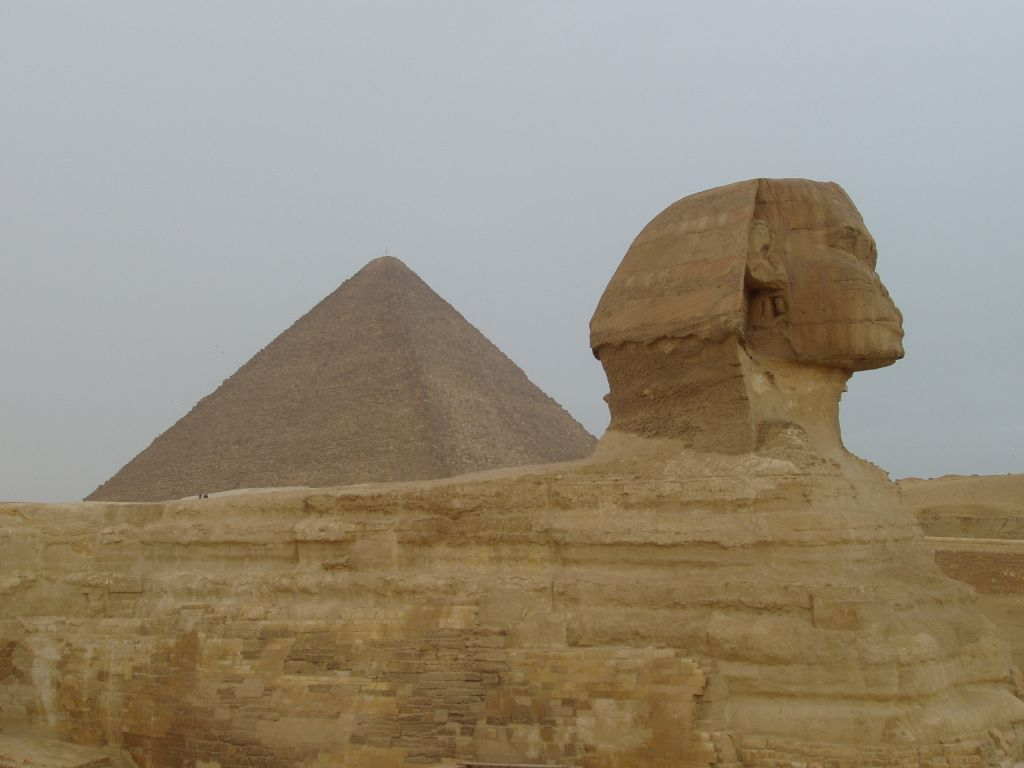
\includegraphics[scale=0.09]{pictures/108103_sm}
	            }
	            \subfigure{
	                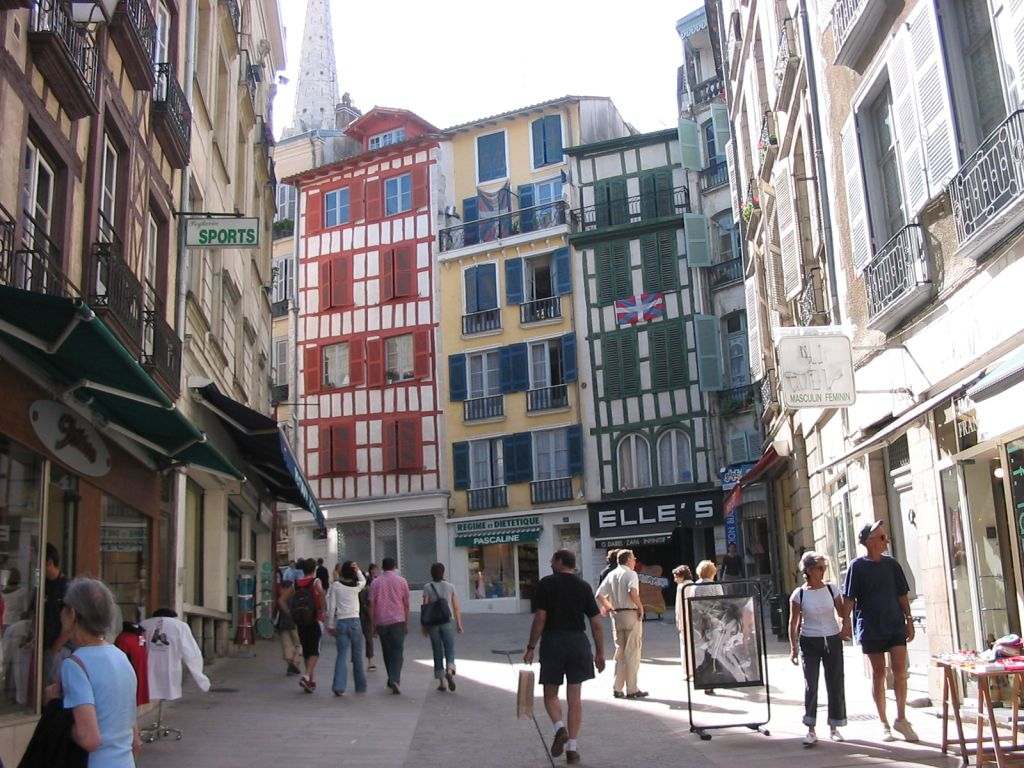
\includegraphics[scale=0.09]{pictures/110701_sm}
	            }
	            \subfigure{
	                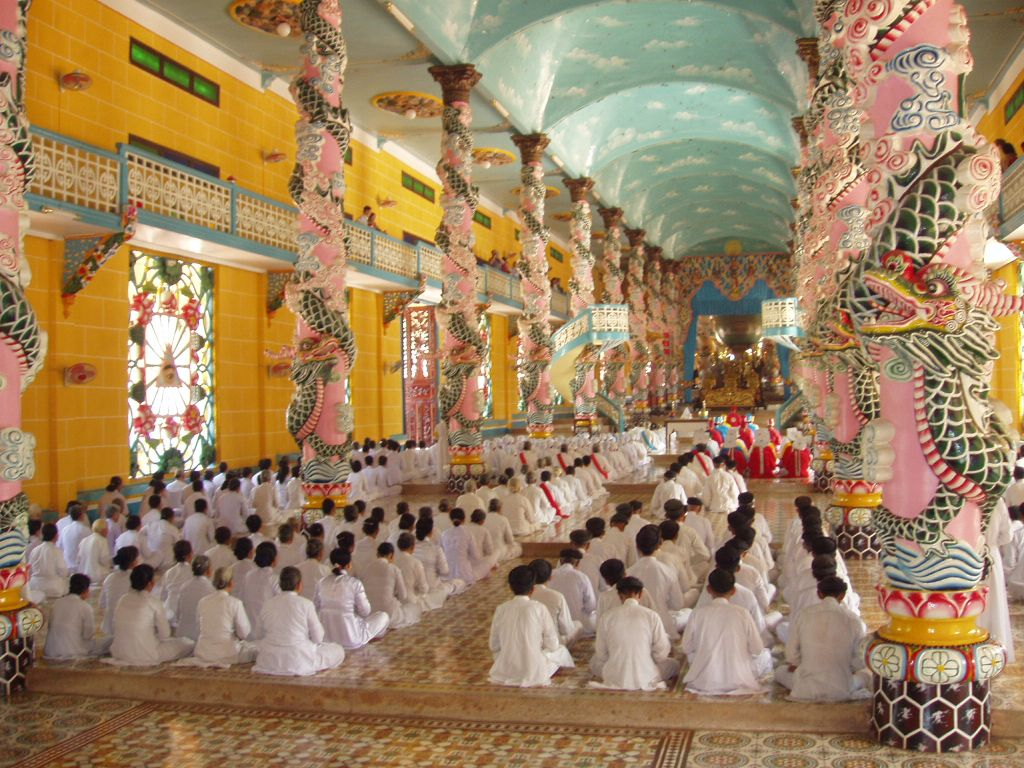
\includegraphics[scale=0.09]{pictures/123205_sm}
	            }
	            \caption{Example images from the INRIA Holidays dataset.}
	        \end{figure}
	    }
	\end{frame}
	
	\begin{frame}{\thesection. Precision-Recall Framework}
	        Precision-Recall curves:
	        \begin{itemize}
	        	\item Recall: ratio of true positives to all related images;
	        	\item Precision: ratio of true positives to number of retrieved images.
	        \end{itemize}
	        \vskip 0.5em
	        
	        \only<1>{
	        	\begin{figure}
	        		\centering
	        		\begin{tikzpicture}
					\begin{axis}[
							height=5cm,
							width=5cm,
							xlabel=Recall,
							ylabel=Precision,
							xtick={0,0.5,1},
							ytick={0,0.5,1},
							ymin=0,
							ymax=1,
							xmin=0,
							xmax=1
						]
						\addplot[RWTHblue,mark=none] coordinates {
							(0,1)
							(0.05,1)
							(0.1,0.95)
							(0.15,0.92)
							(0.2,0.91)
							(0.3,0.91)
							(0.4,0.91)
							(0.5,0.9)
							(0.55,0.9)
							(0.6,0.89)
							(0.65,0.87)
							(0.7,0.8)
							(0.75,0.725)
							(0.8,0.6)
							(0.85,0.25)
							(0.9,0.05)
							(0.95,0)
						};
					\end{axis}
				\end{tikzpicture}
				\begin{tikzpicture}[overlay,remember picture]
			      		\draw[-latex new,arrow head=0.25cm,white,shorten >=3pt,shorten <=3pt,thick,out=45,in=170] (-6,0.25) node{\begin{tabular}{l}area: mean average precision\end{tabular}} (-6,0.5) to (-4,1.25);
		        	\end{tikzpicture}
				%\caption{Precision-Recall curve (schematic plot).}
			\end{figure}
		}
		\only<2>{
			\begin{figure}
	        		\centering
	        		\begin{tikzpicture}
					\begin{axis}[
							height=5cm,
							width=5cm,
							xlabel=Recall,
							ylabel=Precision,
							xtick={0,0.5,1},
							ytick={0,0.5,1},
							ymin=0,
							ymax=1,
							xmin=0,
							xmax=1
						]
						\addplot[fill=RWTHblue,fill opacity=0.25,RWTHblue,mark=none] coordinates {
							(0,1)
							(0.05,1)
							(0.1,0.95)
							(0.15,0.92)
							(0.2,0.91)
							(0.3,0.91)
							(0.4,0.91)
							(0.5,0.9)
							(0.55,0.9)
							(0.6,0.89)
							(0.65,0.87)
							(0.7,0.8)
							(0.75,0.725)
							(0.8,0.6)
							(0.85,0.25)
							(0.9,0.05)
							(0.95,0)
						} -| (current plot begin);
					\end{axis}
				\end{tikzpicture}
				\begin{tikzpicture}[overlay,remember picture]
			      		\draw[-latex new,arrow head=0.25cm,RWTHblue,shorten >=3pt,shorten <=3pt,thick,out=45,in=170] (-6,0.25) node{\begin{tabular}{l}area: mean average precision\end{tabular}} (-6,0.5) to (-3.25,1.25);
		        	\end{tikzpicture}
			    %\caption{Precision-Recall curve (schematic plot).}
			\end{figure}
		}
	\end{frame}
	
	\begin{frame}{\thesection. Experiments}
	    \only<1>{
	        \begin{table}
                \hspace{8em}
                {
                \footnotesize
                \def\arraystretch{1.1}
                \begin{tabular}{| l | r | r |}
                    \hline
                    & Oxford 5k & Holidays\\\hline
                    Fisher Vectors \cite{GordoSerranoPerronninValveny:2012} & -- & 0.774\\
                    Vector of Locally Aggregated Descriptors \cite{ArandjelovicZisserman:2013} & 0.555 & 0.646\\
                    Sparse-Coded Features \cite{GeKeSun:2013} & -- & 0.767\\
                    Triangulation Embedding \cite{JegouZisserman:2014} & 0.676 & 0.771\\\hline
                    \multicolumn{3}{| c |}{\textbf{Pre-Trained on ImageNet}}\\\hline
                    $l = 10$ & 0.389 & 0.69\\
                    $l = 11$ & 0.435 & 0.749\\
                    $l = 12$ & 0.430 & 0.736\\\hline
                    \multicolumn{3}{| c |}{\textbf{Re-Trained}}\\\hline
                    $l = 10$ & 0.387 & 0.674\\
                    $l = 11$ & 0.545 & 0.793\\
                    $l = 12$ & 0.538 & 0.764\\\hline
                \end{tabular}
                }
                \caption{Mean average precision for the Oxford 5k dataset and the Holidays dataset.}
                \label{table:pre-re-trained}
            \end{table}
        }
        \only<2>{
            \begin{table}
                \hspace{8em}
                {
                \footnotesize
                \def\arraystretch{1.1}
                \begin{tabular}{| l | r | r |}
                    \hline
                    & Oxford 5k & Holidays\\\hline
                    Fisher Vectors \cite{GordoSerranoPerronninValveny:2012} & -- & 0.774\\
                    Vector of Locally Aggregated Descriptors \cite{ArandjelovicZisserman:2013} & 0.555 & 0.646\\
                    Sparse-Coded Features \cite{GeKeSun:2013} & -- & 0.767\\
                    Triangulation Embedding \cite{JegouZisserman:2014} & \textbf{0.676} & 0.771\\\hline
                    \multicolumn{3}{| c |}{\textbf{Pre-Trained on ImageNet}}\\\hline
                    $l = 10$ & \textcolor{RWTHblue}{0.389} & 0.69\\
                    $l = 11$ & \textcolor{RWTHblue}{0.435} & 0.749\\
                    $l = 12$ & \textcolor{RWTHblue}{0.430} & 0.736\\\hline
                    \multicolumn{3}{| c |}{\textbf{Re-Trained}}\\\hline
                    $l = 10$ & \textcolor{RWTHblue}{0.387} & 0.674\\
                    $l = 11$ & \textcolor{RWTHblue}{0.545} & 0.793\\
                    $l = 12$ & \textcolor{RWTHblue}{0.538} & 0.764\\\hline
                \end{tabular}
                }
                \caption{Mean average precision for the Oxford 5k dataset and the Holidays dataset.}
                \label{table:pre-re-trained}
            \end{table}
        }
        \only<3>{
            \begin{table}
                \hspace{8em}
                {
                \footnotesize
                \def\arraystretch{1.1}
                \begin{tabular}{| l | r | r |}
                    \hline
                    & Oxford 5k & Holidays\\\hline
                    Fisher Vectors \cite{GordoSerranoPerronninValveny:2012} & -- & 0.774\\
                    Vector of Locally Aggregated Descriptors \cite{ArandjelovicZisserman:2013} & 0.555 & 0.646\\
                    Sparse-Coded Features \cite{GeKeSun:2013} & -- & 0.767\\
                    Triangulation Embedding \cite{JegouZisserman:2014} & 0.676 & 0.771\\\hline
                    \multicolumn{3}{| c |}{\textbf{Pre-Trained on ImageNet}}\\\hline
                    $l = 10$ & 0.389 & \textcolor{RWTHblue}{0.69}\\
                    $l = 11$ & 0.435 & \textcolor{RWTHblue}{0.749}\\
                    $l = 12$ & 0.430 & \textcolor{RWTHblue}{0.736}\\\hline
                    \multicolumn{3}{| c |}{\textbf{Re-Trained}}\\\hline
                    $l = 10$ & 0.387 & \textcolor{RWTHblue}{0.674}\\
                    $l = 11$ & 0.545 & \textcolor{RWTHblue}{\textbf{0.793}}\\
                    $l = 12$ & 0.538 & \textcolor{RWTHblue}{0.764}\\\hline
                \end{tabular}
                }
                \caption{Mean average precision for the Oxford 5k dataset and the Holidays dataset.}
                \label{table:pre-re-trained}
            \end{table}
        }
	\end{frame}
	
	\begin{frame}{\thesection. Experiments with Compression}
	    \only<1>{
	        \begin{table}
                \hspace{8em}
                {
                \footnotesize
                \def\arraystretch{1.1}
                \begin{tabular}{| l | r | r |}
                    \hline
                    & Oxford 5k & Holidays\\\hline
                    Fisher Vectors \cite{GordoSerranoPerronninValveny:2012} & -- & 0.723\\
                    Fisher Vectors* \cite{GordoSerranoPerronninValveny:2012} & -- & 0.764\\
                    Vector of Locally Aggregated Descriptors \cite{ArandjelovicZisserman:2013} & 0.448 & 0.625\\
                    Sparse-Coded Features \cite{GeKeSun:2013} & -- & 0.727\\
                    Triangulation Embedding \cite{JegouZisserman:2014} & 0.433 & 0.617\\\hline
                    \multicolumn{3}{| c |}{\textbf{Pre-Trained on ImageNet}}\\\hline
                    $l = 11$ (PCA) & 0.433 & 0.747\\
                    $l = 11$ (Large-Margin) & 0.439 & --\\\hline
                    \multicolumn{3}{| c |}{\textbf{Re-Trained}}\\\hline
                    $l = 11$ (PCA)& 0.557 & 0.789\\
                    \hline
                \end{tabular}
                }
                \caption{Mean average precision for the Oxford 5k dataset and the Holidays dataset using $128$ dimensional image representations.}
                \label{table:compression}
            \end{table}
        }
        \only<2>{
            \begin{table}
                \hspace{8em}
                {
                \footnotesize
                \def\arraystretch{1.1}
                \begin{tabular}{| l | r | r |}
                    \hline
                    & Oxford 5k & Holidays\\\hline
                    Fisher Vectors \cite{GordoSerranoPerronninValveny:2012} & -- & 0.723\\
                    Fisher Vectors* \cite{GordoSerranoPerronninValveny:2012} & -- & 0.764\\
                    Vector of Locally Aggregated Descriptors \cite{ArandjelovicZisserman:2013} & 0.448 & 0.625\\
                    Sparse-Coded Features \cite{GeKeSun:2013} & -- & 0.727\\
                    Triangulation Embedding \cite{JegouZisserman:2014} & 0.433 & 0.617\\\hline
                    \multicolumn{3}{| c |}{\textbf{Pre-Trained on ImageNet}}\\\hline
                    $l = 11$ (PCA) & \textcolor{RWTHblue}{0.433} & 0.747\\
                    $l = 11$ (Large-Margin) & \textcolor{RWTHblue}{0.439} & --\\\hline
                    \multicolumn{3}{| c |}{\textbf{Re-Trained}}\\\hline
                    $l = 11$ (PCA)& \textcolor{RWTHblue}{\textbf{0.557}} & 0.789\\
                    \hline
                \end{tabular}
                }
                \caption{Mean average precision for the Oxford 5k dataset and the Holidays dataset using $128$ dimensional image representations.}
                \label{table:compression}
            \end{table}
        }
        \only<3>{
            \begin{table}
                \hspace{8em}
                {
                \footnotesize
                \def\arraystretch{1.1}
                \begin{tabular}{| l | r | r |}
                    \hline
                    & Oxford 5k & Holidays\\\hline
                    Fisher Vectors \cite{GordoSerranoPerronninValveny:2012} & -- & 0.723\\
                    Fisher Vectors* \cite{GordoSerranoPerronninValveny:2012} & -- & 0.764\\
                    Vector of Locally Aggregated Descriptors \cite{ArandjelovicZisserman:2013} & 0.448 & 0.625\\
                    Sparse-Coded Features \cite{GeKeSun:2013} & -- & 0.727\\
                    Triangulation Embedding \cite{JegouZisserman:2014} & 0.433 & 0.617\\\hline
                    \multicolumn{3}{| c |}{\textbf{Pre-Trained on ImageNet}}\\\hline
                    $l = 11$ (PCA) & 0.433 & \textcolor{RWTHblue}{0.747}\\
                    $l = 11$ (Large-Margin) & 0.439 & \textcolor{RWTHblue}{--}\\\hline
                    \multicolumn{3}{| c |}{\textbf{Re-Trained}}\\\hline
                    $l = 11$ (PCA)& 0.557 & \textcolor{RWTHblue}{\textbf{0.789}}\\
                    \hline
                \end{tabular}
                }
                \caption{Mean average precision for the Oxford 5k dataset and the Holidays dataset using $128$ dimensional image representations.}
                \label{table:compression}
            \end{table}
        }
	\end{frame}
	
	\begin{frame}{\thesection. Experiments -- Examples}
	    \begin{figure}
	        \hspace{4em}
	        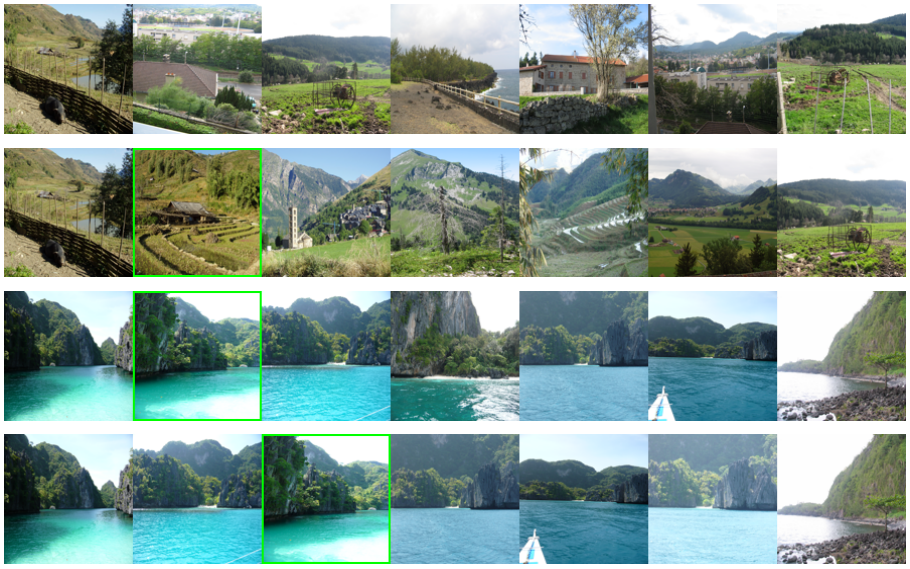
\includegraphics[scale=0.3]{pictures/qualitative}
	        \begin{tikzpicture}[overlay,remember picture]
	            \draw[RWTHblue] (-10.75,5.25) node{\begin{tabular}{l}pre-trained\end{tabular}};
	            \draw[RWTHblue] (-10.75,3.75) node{\begin{tabular}{l}re-trained\end{tabular}};
	            \draw[RWTHblue] (-10.75,2.25) node{\begin{tabular}{l}pre-trained\end{tabular}};
	            \draw[RWTHblue] (-10.75,0.75) node{\begin{tabular}{l}re-trained\end{tabular}};
            \end{tikzpicture}
            \caption{Qualitative examples provided by Babenko et al. \cite{BabenkoSlesarevChigorinLempitsky:2014}: left-most image is the query; correctly retrieved images are marked.}
	    \end{figure}
	\end{frame}
	
    \begin{frame}{\thesection. Experiments -- Conclusion}
	    Notes on Experiments:
	    \begin{itemize}
	        \item no experiments using Large Margin Dimensionality Reduction on the re-trained model;
	        \item and the results for state-of-the-art approaches are taken from the corresponding publications.
	    \end{itemize}
	    \vskip 0.5em
	    \pause
	    
	    Conclusion:
	    \begin{itemize}
	        \item fully learned features are interesting alternative to hand-crafted features;
	        \item and convolutional neural networks may be explicitly trained for the image retrieval task.
	    \end{itemize}
	\end{frame}	
	
	\section{Summary}
	\begin{frame}{\thesection. Summary}
	    Summary and takeaways:
	    \begin{enumerate}[1.]
	        \item State-of-the-art image retrieval techniques aggregate local descriptors:
	        \begin{itemize}
	            \item Bag of Visual Words \cite{SivicZisserman:2003};
	            \item Vector of Locally Aggregated Gradients \cite{ArandjelovicZisserman:2013};
	            \item Sparse-Coded Features \cite{GeKeSun:2013}.
	        \end{itemize}
	        \pause
	        \item Convolutional neural networks are powerful, but complex models for classification.
	        \begin{itemize}
	            \item Excellent performance on ImageNet;
	            \item but difficult to train or implement.
	        \end{itemize}
	        \pause
	        \item Intermediate feature activations of convolutional neural networks offer rich representations.
	    \end{enumerate}
	\end{frame}
	
	\begin{appendix}
	    \begin{frame}{A.1. Bag of Visual Words -- Discussion}
		    % Extensions: term-frequency and inverse document frequency weighting.
	        % \vskip 0.5em
	        
	        For large $Y$, $k$-means clustering may be infeasible:
	        \begin{itemize}
	            \item hierarchical $k$-means \cite{NisterStewenius:2006};
	            \item or approximate $k$-means \cite{PhilbinChumIsardSivicZisserman:2007}.
	        \end{itemize}
	        \vskip 1.5em
	        
	        Burstiness, that is single large components can strongly affect performance \cite{ArandjelovicZisserman:2013}:
	        \begin{itemize}
	            \item term frequency, inverse document frequency weighting;
	            \item or component-wise square root and $L_2$ normalization.
	        \end{itemize}
	    \end{frame}
	    
	    \begin{frame}{A.2. Vector of Locally Aggregated Descriptors}
	        Remember, embedding step:
		    \begin{align*}
                f(y_{l,n}) = \left(\delta(\text{NN}_{\hat{Y}}(y_{l,n}) = \hat{y}_1)(y_{l,n} - \hat{y}_1),\ldots\right),
            \end{align*}
	        and aggregation step:
            \begin{align*}
		        F(Y_n) = \sum_{l = 1}^L f(y_{l,n}).
	        \end{align*}
	        \vskip 0.5em
	        
	        Further normalization techniques:
	        \begin{itemize}
	            \item power-law normalization (usually, $\alpha = 0.5$):
	            \begin{align*}
	                F_m(Y_n) = \text{sign}\left(F_m(Y_n)\right) \left|F_m(Y_n)\right|^\alpha;
	            \end{align*}
	            \item intra-normalization: $L_2$-normalize sum of residuals for each visual word independently.
	        \end{itemize}
	    \end{frame}
	    
	    \begin{frame}{B. Training in Practice}
	        Training with gradient descent, in iteration $[t + 1]$ compute
	        \begin{align*}
	            W[t + 1] = W[t] - \gamma \nabla E(W[t])
	        \end{align*}
	        with learning rate $\gamma$.
	        \vskip 0.5em
	        
	        In practice:
	        \begin{itemize}
	            \item Compute $\nabla E(W[t])$ in $\mathcal{O}(|W|)$ using Error Backpropagation.
	            \item Add a regularizer of the form
	                \begin{align*}
	                    \hat{E}(W) = E(W) + \lambda \|W\|_1.
	                \end{align*}
	            \item Use dropout \cite{HintonSrivastavaKrizhevskySutskeverSalakhutdinoc:2012} and stochastic gradient descent.
	        \end{itemize}
	    \end{frame}
	    
	    \begin{frame}{C. Neural Codes -- Motivation}
	        \begin{figure}
	            \subfigure{
	                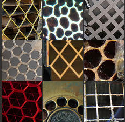
\includegraphics[scale=1]{pictures/layer-3}
	            }
	            \subfigure{
	                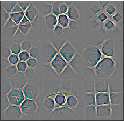
\includegraphics[scale=1]{pictures/layer-3-activations}
	            }
	            \caption{Back-projection of a single feature activation in layer $l=3$ \cite{ZeilerFergus:2014}\footnotemark.}
	        \end{figure}
	        \footnotetext{Note that the architecture used by Zeiler et al. \cite{ZeilerFergus:2014} does not exactly match the architecture presented previously.}
	    \end{frame}
	
	    \begin{frame}{C. Neural Codes -- Motivation}
	        \begin{figure}
	            \subfigure{
	                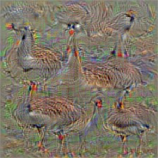
\includegraphics[scale=0.65]{pictures/goose}
	            }
	            \subfigure{
	                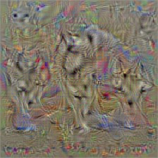
\includegraphics[scale=0.65]{pictures/husky}
	            }
	            \caption{Computed image to maximize posterior for classes ``goose'' (left) and ``husky'' (right) \cite{SimonyanVedaldiZisserman:2013}.}
	        \end{figure}
	    \end{frame}
	    
	    \begin{frame}{D. Try it out ...}
	        Unfortunately, Babenko et al. do not provide source code to reproduce their experiments.
	        \vskip 0.5em
	        
	        However, you can try other state-of-the-art approaches:
	        \begin{itemize}
	            \item Oxford 5k dataset (including evaluation script): \url{http://www.robots.ox.ac.uk/~vgg/data/oxbuildings/};
	            \item SIFT, Vector of Locally Aggregated Descriptors and Fisher Vectors \cite{PerronninDance:2007} are implemented in the VLFeat library: \url{http://www.vlfeat.org/overview/encodings.html};
	        \end{itemize}
	        \vskip 0.5em
	        
	        ... or try to use convolutional neural networks, for example using
	        \begin{itemize}
	            \item Caffe: \url{http://caffe.berkeleyvision.org/}.
	        \end{itemize}
	    \end{frame}
	\end{appendix}
	
	\bibliographystyle{alpha}
	\bibliography{slides}
	
\end{document}
